\section{Possibili malfunzionamenti}

È possibile che l'applicazione abbia dei malfunzionamenti. Ci sono quattro possibili casi:
	\begin{enumerate}
		\item Al momento dell'apertura dell'applicazione il dispositivo non è connesso alla rete. In questo caso viene visualizzato un messaggio di errore e l'applicazione viene chiusa;
		\item Durante l'utilizzo dell'applicazione, il dispositivo perde la connettività. In questo caso viene visualizzato un messaggio d'errore che invita l'utente ad attendere il ripristino della connessione prima di eseguire altre operazioni;
		\item In fase di login non è possibile raggiungere le informazioni su articoli e ordini dell'azienda fornitrice. In questo caso viene visualizzato un messaggio d'errore che informa l'utente della presenza di un'inconsistenza nel database di VISIONIMPRESA;
		\item Prima del completo caricamento di una pagina l'utente clicca su qualche oggetto. In questi casi può succedere che l'app non abbia il comportamento atteso. La velocità del caricamento dipende della velocità della connessione Internet, per cui si invita l'utente ad attendere la scomparsa dell'animazione di caricamento, prima di effettuare operazioni.
	\end{enumerate}
	
\begin{figure}[h]

\centering
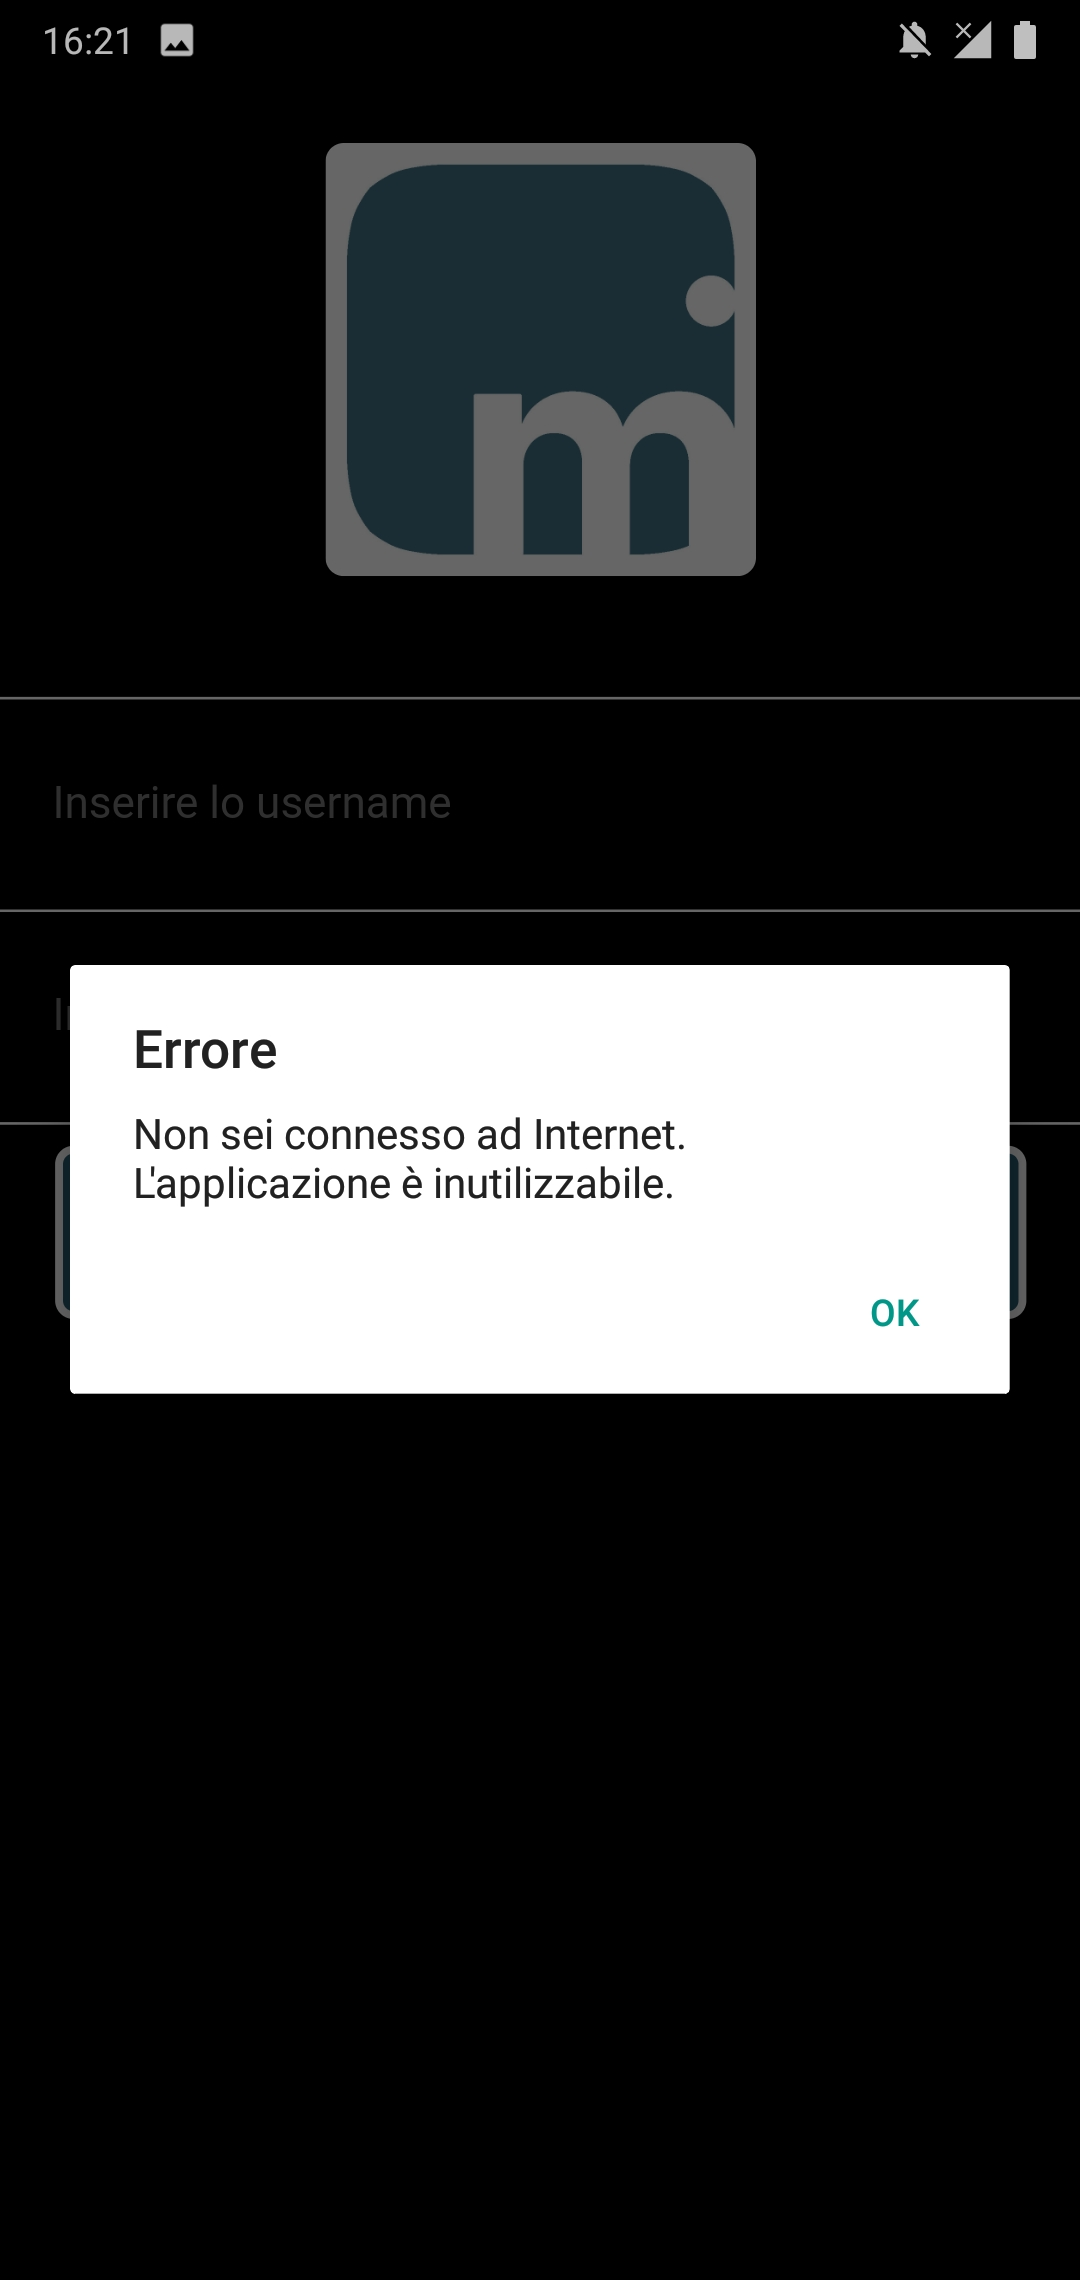
\includegraphics[width=.3\textwidth]{./img/erroreInternet.jpg}\hfill
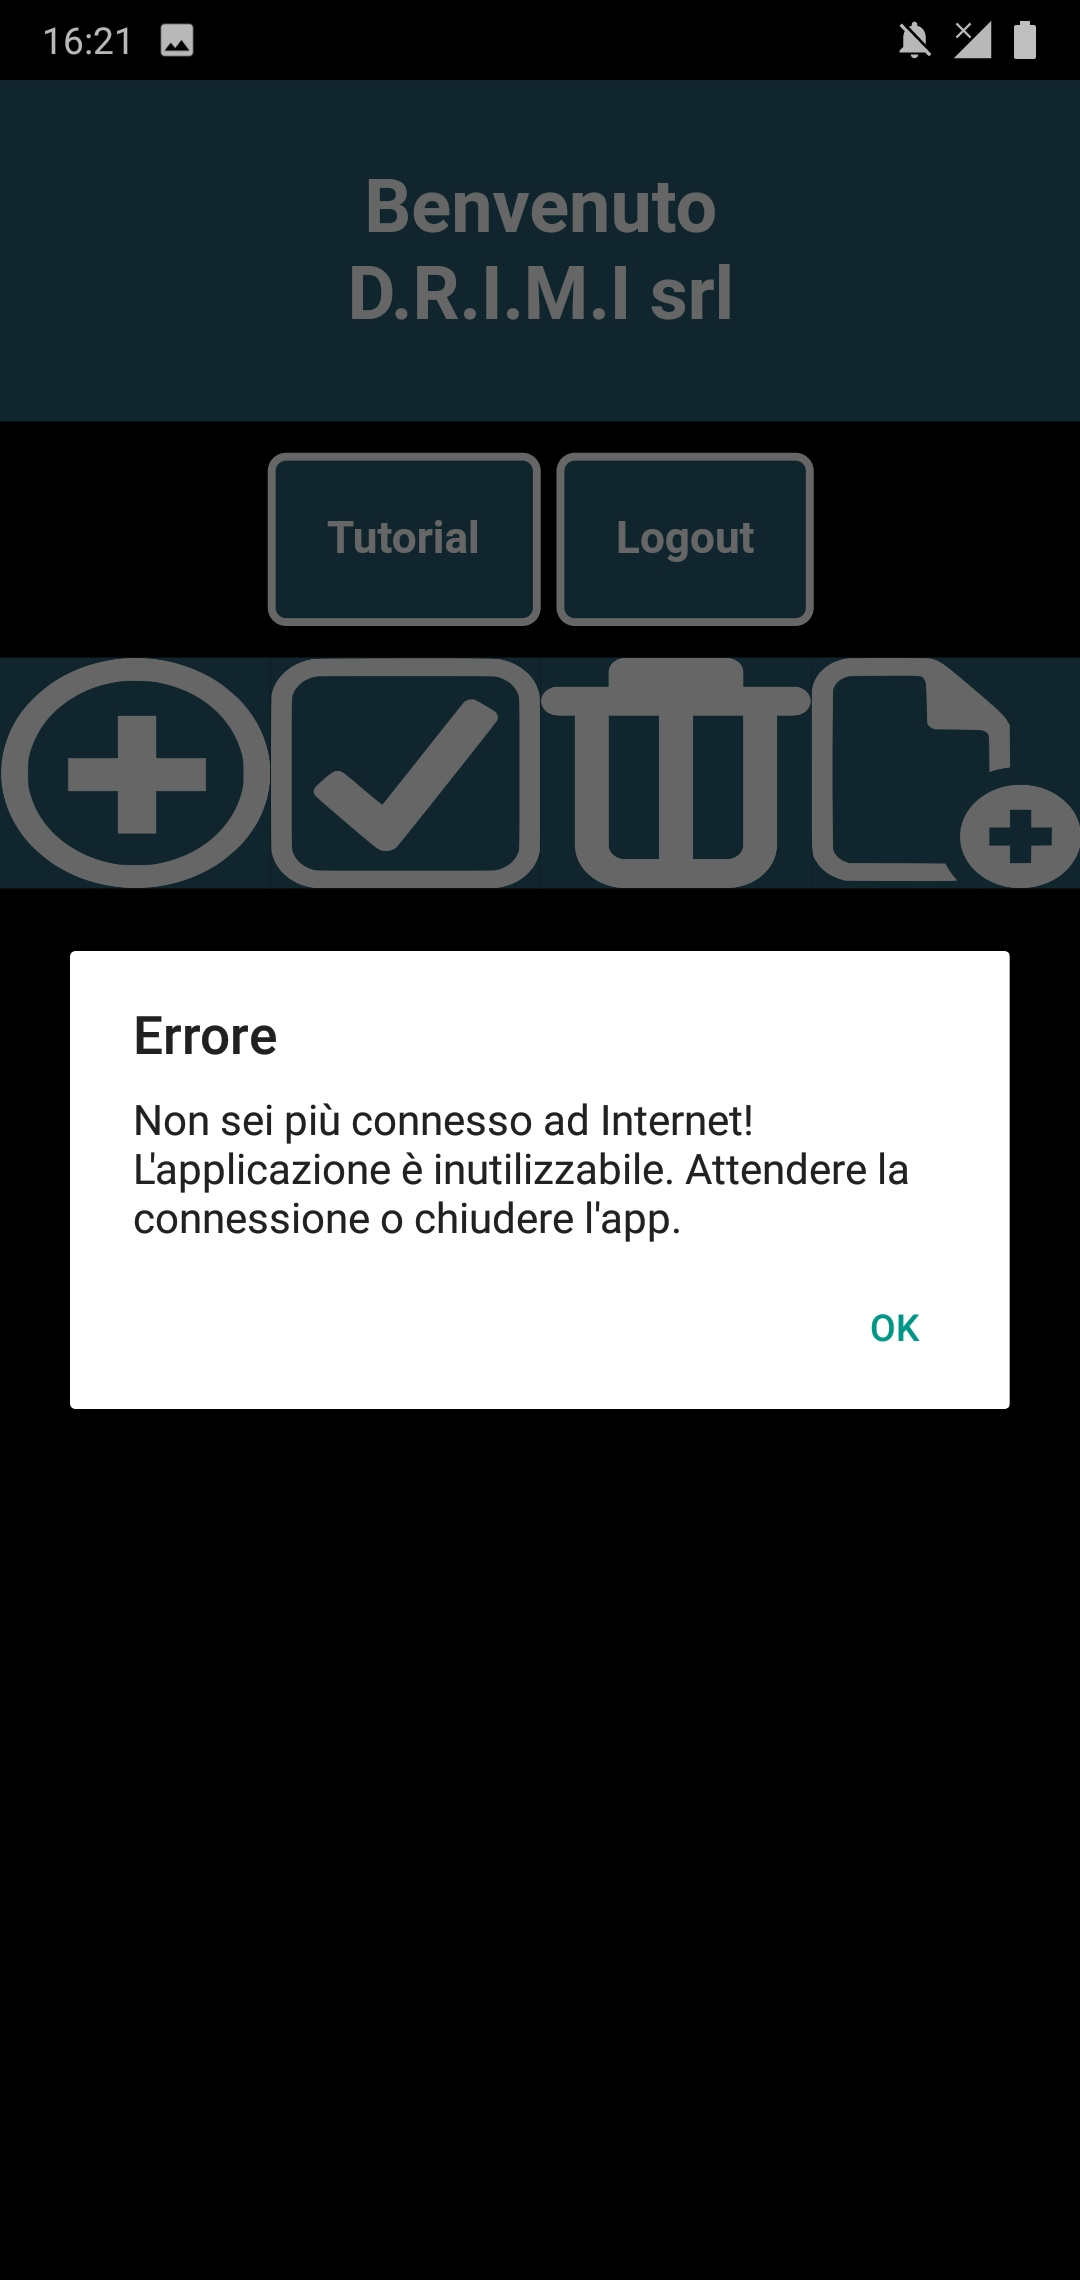
\includegraphics[width=.3\textwidth]{./img/erroreInternet2.jpg}\hfill
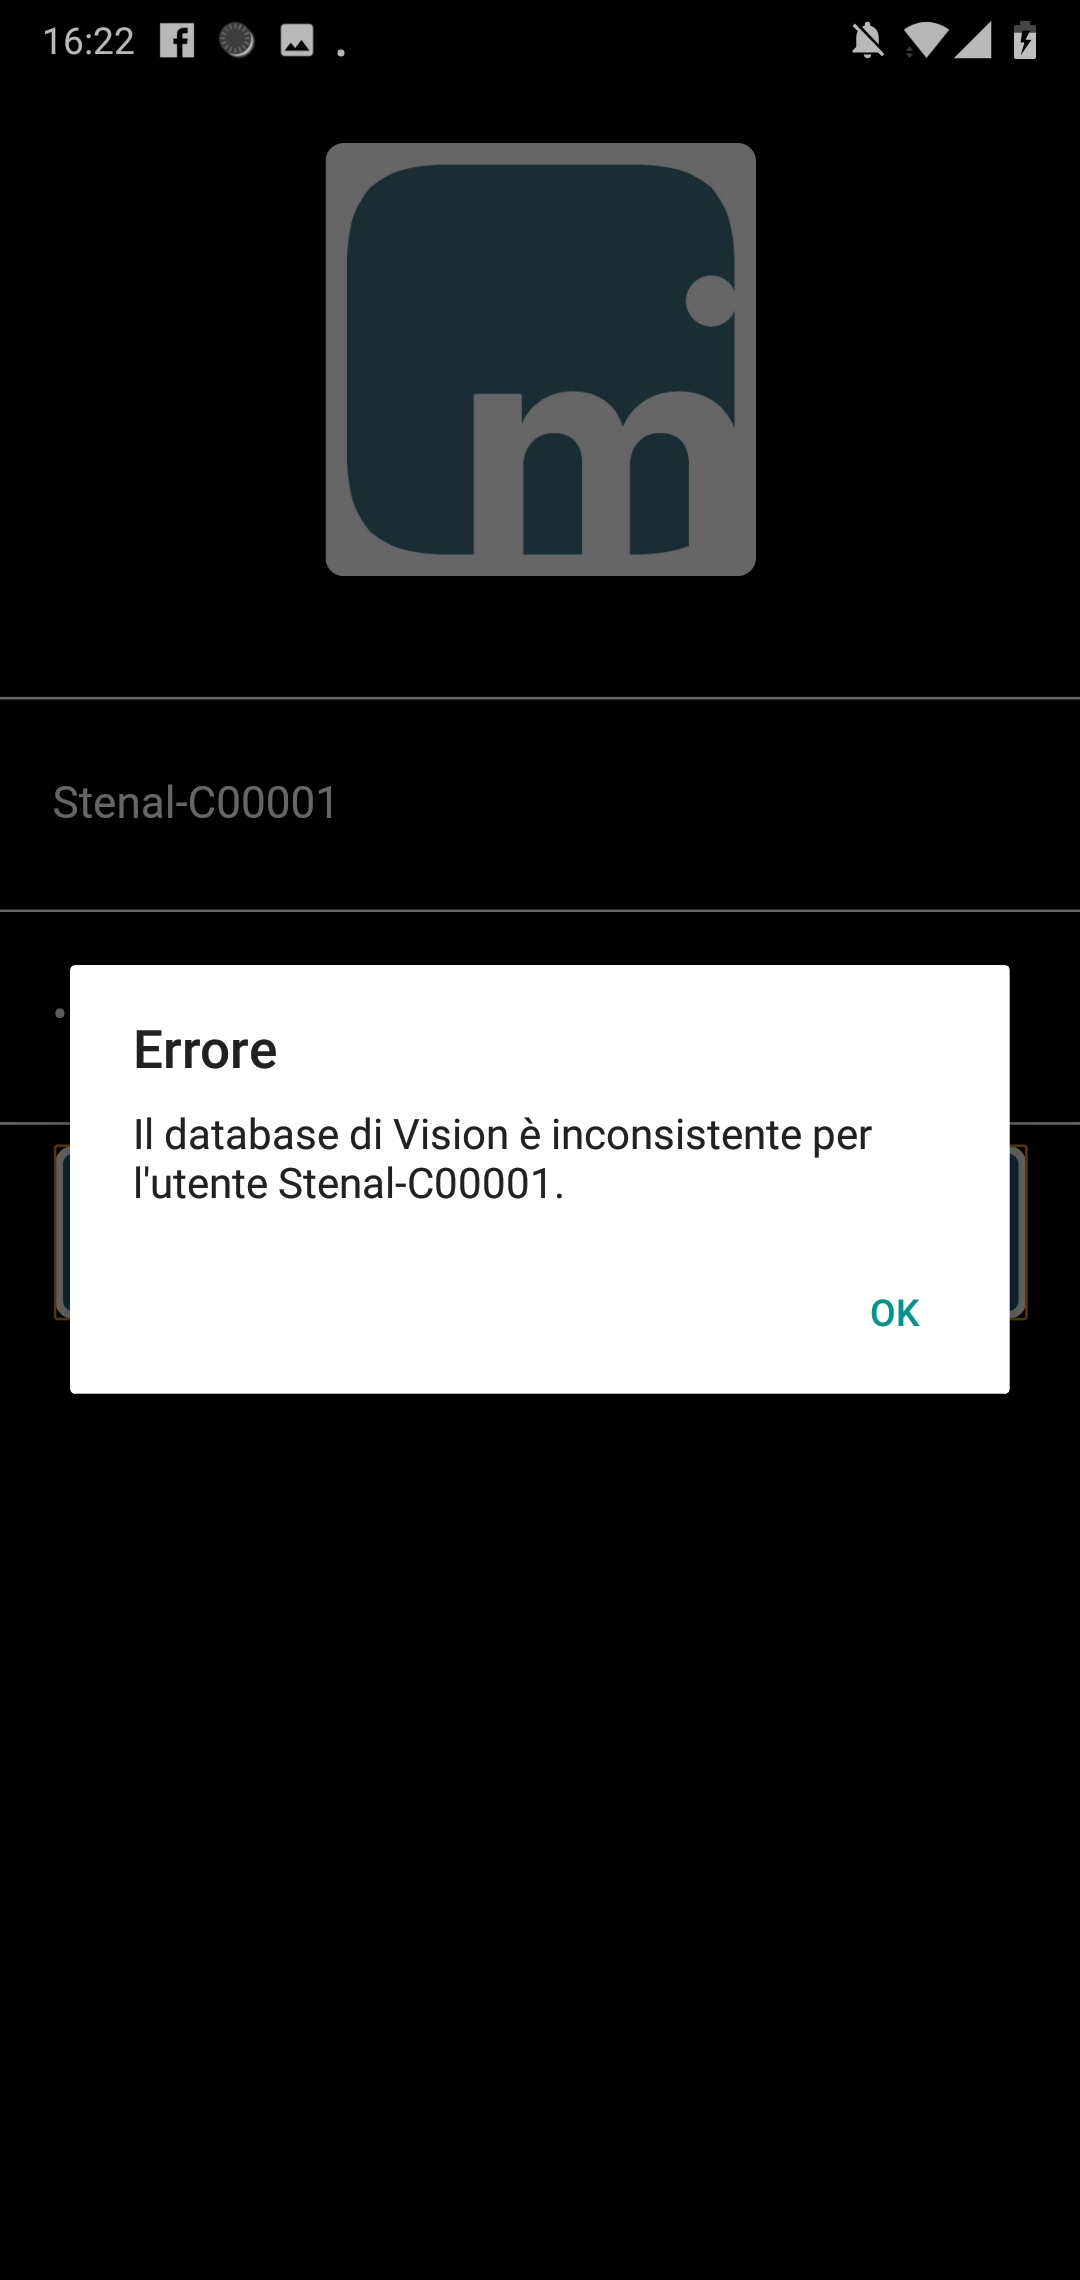
\includegraphics[width=.3\textwidth]{./img/erroreDB.jpg}

\caption[Possibili errori dell'applicazione]{A sinistra la prima tipologia di errore di connessione, al centro la seconda tipologia di errore di connessione, a destra l'errore di accesso al database dell'azienda}

\end{figure}